\noindent Para hallar el punto $B' \in \alpha$ y cuya distancia a $B$ es igual a la distancia de $B$ a $\alpha$ podemos hacer uso del vector proyección $\vec{p}$ antes mencionado para luego restarlo del vector $\vec{b}$, lo que nos da como resultado un vector $\vec{b'}$ cuyo sentido (punta flecha) coincidirá con el punto $B' \in \alpha$:
\begin{center}
	$\boxed{\vec{p} = \cfrac{\vec{b} \cdot \vec{n}}{|\vec{n}|^2} \cdot \vec{n}} \hspace*{1cm}
		\vec{n}=(3, 2, -5)  \hspace*{1cm}
		\vec{b}=(2, 1, -1) \hspace*{1cm}
		\vec{b} \cdot \vec{n}  = 13 \hspace*{1cm}
		|\vec{n}|  = \sqrt{38}$
\end{center}
\begin{multicols}{2}
	\noindent Calculamos $\vec{p}$:
	\begin{align*}
		\vec{p} & = \cfrac{\vec{b} \cdot \vec{n}}{|\vec{n}|^2} \cdot \vec{n}       \\
		\vec{p} & = \cfrac{13}{(\sqrt{38})^2} \cdot (3, 2, -5)                     \\
		\vec{p} & = \cfrac{13}{38} \cdot (3, 2, -5)                                \\
		\vec{p} & = \left( \cfrac{39}{38}, \cfrac{26}{38}, -\cfrac{65}{38} \right) \\
	\end{align*}
	\noindent Calculamos $\vec{b'}$:
	\begin{align*}
		\vec{b'} & = \vec{b} - \vec{p}                                                           \\
		\vec{b'} & = (2, 1, -1) - \left( \cfrac{39}{38}, \cfrac{26}{38}, -\cfrac{65}{38} \right) \\
		\vec{b'} & = \left( 2 - \cfrac{39}{38}, 1 - \cfrac{26}{38}, -1 + \cfrac{65}{38} \right)  \\
		\vec{b'} & = \left( \cfrac{37}{38}, \cfrac{12}{38}, \cfrac{27}{38} \right)
	\end{align*}
\end{multicols}

\noindent $\therefore$ \ Las coordenadas del punto $B'$ que está contenido en $\alpha$ y cuya distancia a $B$ es igual a la distancia de $B$ a $\alpha$ es:

\fcolorbox{black}{yellow}{$B'\left( \cfrac{37}{38}, \cfrac{12}{38}, \cfrac{27}{38} \right)$}
\ $\approx \ (0.974; \ 0.316;\ 0.711)$

\newpage
\noindent \textbf{Gráfica 18-a,b}:
\begin{center}
	\href{https://www.geogebra.org/3d/wrk3eabw}{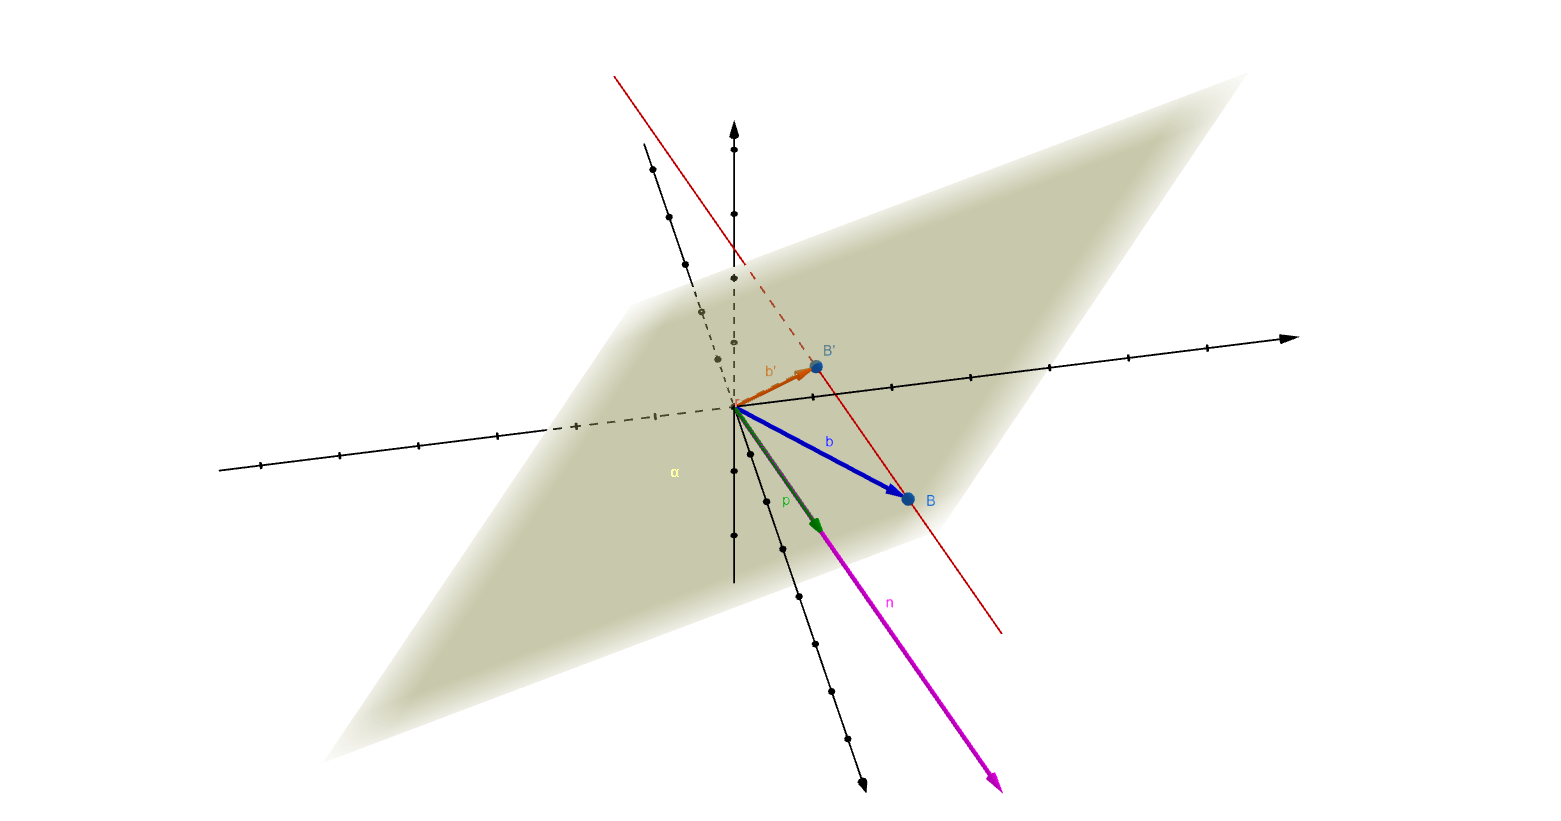
\includegraphics[width=15cm, scale=1]{TP-MATEMATICA-EJ18AB.png}}
\end{center}

